% !TEX root=../master.tex
\chapter{Results}
\label{ch:results}


\section{Simulation Setup}
In order to test the full system, we simulated the handoff scenario using Gazebo 7 and ROS. While a hardware demonstration is preferrable, we were able to show a fully working system with simulated noise in software, suggesting that with minor tweaks and tuning, the methods described here would result in a successful hardware implementation.

The aircraft dynamics were simulated according to the framework presented in~\cite{BeardMcLain12}, with parameters for a small fixed-wind UAV. The ground targets are represented by pedestrians that wander randomly within a 140m by 270m area. In order to provide visual features, a satellite image of a rural area is used as the ground plane for the simulated world.

\begin{figure}[hbt]
  \centering
  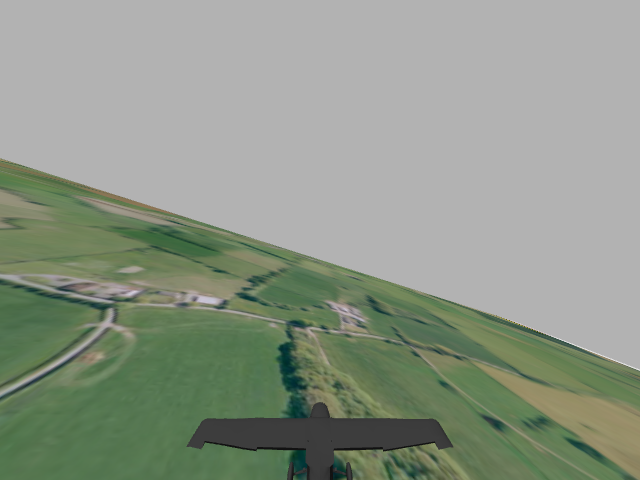
\includegraphics[width=1.0\columnwidth]{figures/sim_chase}
  \caption{Snapshot of the handoff vehicle orbiting about the target above a simulated rural ground plane.}
  \label{fig:sim_chase}
\end{figure}

Each UAV is equipped with IMU and magnetometer sensor plugins and the range sensor used in the relative pose estimator from Chapter~\ref{ch:relative_pose} is simulated by computing the norm of the distance between the two UAVs, with zero-mean Gaussian noise.
Each vehicle also has a camera with a two-axis gimbal.

Becuase the visual from the camera is not directly linked to the targets, it makes it difficult to establish a test to determine with aboslute certainty if the handoff vehicle associates the correct track with the true target.
To overcome this issue, we simulated the camera and tracking information by projecting the positions of the targets into the camera frame of the UAV with noise added to the LOS and camera frame pixel positions.

For simplicity, both UAVs are deployed simultaneously, but the tracking UAV uses absolute position to navigate directly to the target, while the handoff UAV begins estimating the relative pose between aircraft to determine the target's location.
The handoff UAV is able to successfully determine the relative pose between the aircraft and insert into a similar orbit.
As the targets enter the handoff vehicle's field of view, the handoff UAV begins tracking each target and, over time, gains sufficient confidence to complete the handoff.
The handoff vehicle continues to track and orbit the target using only visual information.

\section{Results}
We ran the simulation 500 times and measured the time it took for the handofff vehicle to complete the handoff and whether or not it selected the correct target among 5 different randomly moving targets. We considered it a failure if the UAV couldn't determine the correct target within 15 minutes. The UAV was able to accurately determine the correct target 97.2\% of the time time with an average handoff time of 314 seconds.

We also conducted monte carlo simulations to test the limitations of our approach and to evaluate some of the tradeoffs of certain parameters. The main tradeoff we identified was the time it took the handoff vehicle to make a decision vs. the accuracy of that decision. The handoff logic thresholds and the track comparison window size seemed to be the primary determining factors for this tradeoff. As the requirements for handoff become more difficult to meet, namely lower thresholds and larger window sizes, the accuracy of the handoff increases, but it also takes increasingly long to make a decision. To characterize this tradeoff between the speed of the decision and the accuracy, we varied both the window size and the residual threshold. We ran 100 iterations of each parameter configuration and average the results. Figure~\ref{fig:sim_time_vs_accuracy}-\ref{fig:sim_threshold_vs_time} show the trends observed for various window size and threshold parameters.

\begin{figure}[hbt]
  \centering
  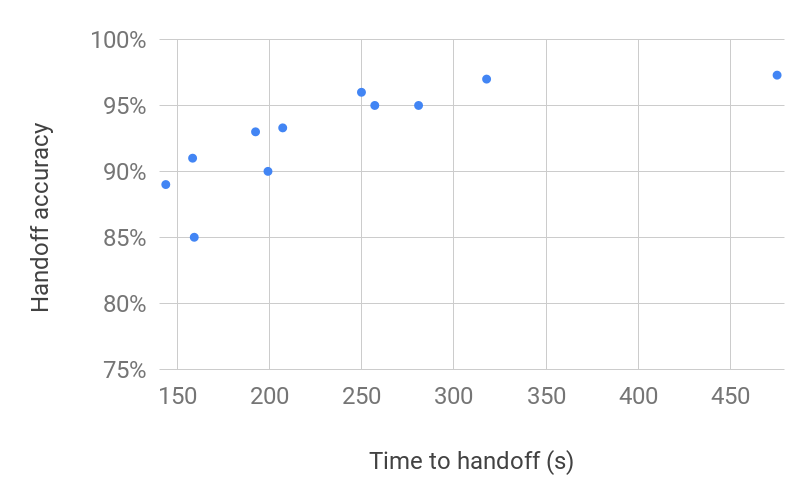
\includegraphics[width=0.7\columnwidth]{figures/sim_time_vs_accuracy}
  \caption{Positive relationship between the time to handoff and handoff accuracy for various window size and threshold values. }
  \label{fig:sim_time_vs_accuracy}
\end{figure}

If the window size was too small or the threshold too high, then the accuracy suffered. The handoff vehicle would make a decision sooner, but it was less likely  to make the correct decision. As the window size increased and the threshold lowered, the conditions for handoff were more stringent and accordingly, accuracy went up. As the accuracy exceeded 97\%, the time it took the handoff vehicle to make a decision increased significantly. Using a window size of 100 and residual threshold of 15 meters seemed to provide a reasonable balance, giving 97.2\% accuracy and a handoff time of 314 seconds, as described above.
\begin{figure}[hbt]
  \centering
  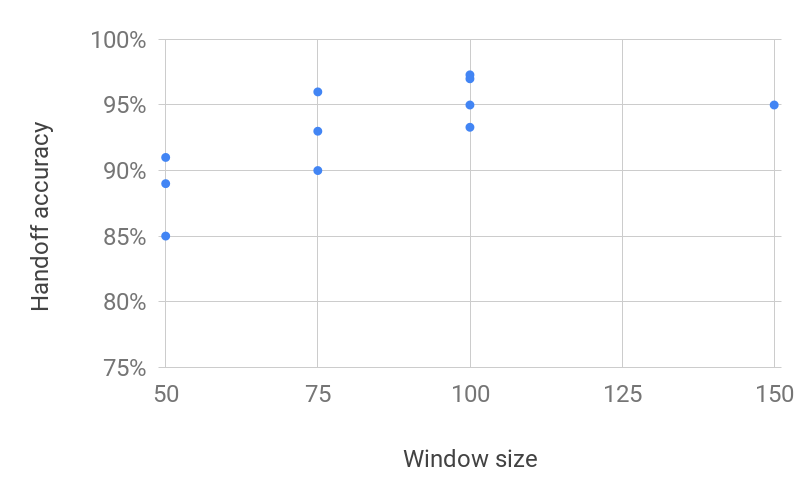
\includegraphics[width=0.7\columnwidth]{figures/sim_window_vs_accuracy}
  \caption{Positive relationship between the handoff logic window size and handoff accuracy for various threshold values.}
  \label{fig:sim_window_vs_accuracy}
\end{figure}

\begin{figure}[hbt]
  \centering
  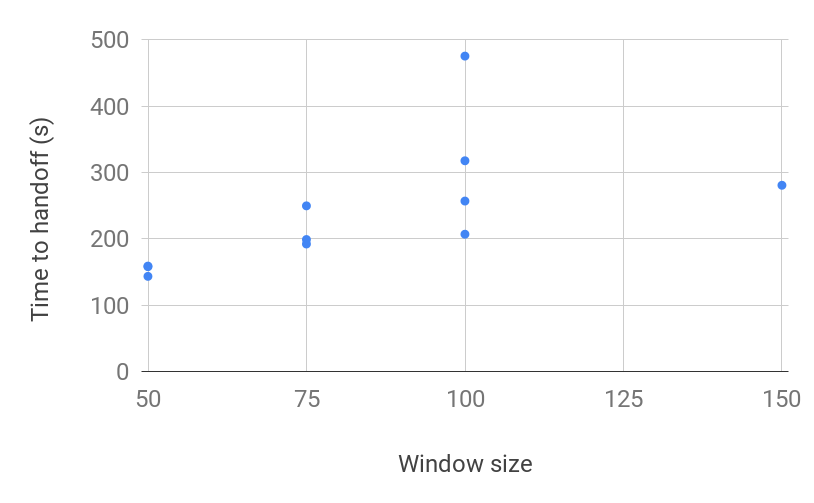
\includegraphics[width=0.7\columnwidth]{figures/sim_window_vs_time}
  \caption{Positive relationship between the handoff logic window size and the time to handoff for various threshold values.}
  \label{fig:sim_window_vs_time}
\end{figure}

\begin{figure}[hbt]
  \centering
  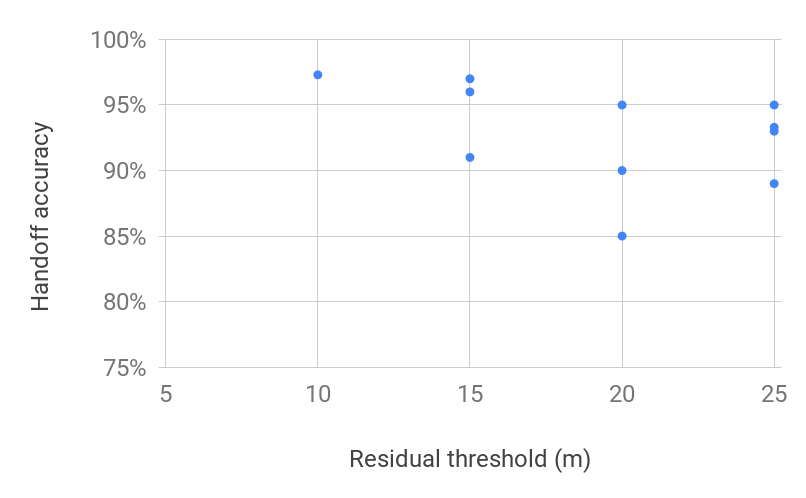
\includegraphics[width=0.7\columnwidth]{figures/sim_threshold_vs_accuracy}
  \caption{Negative relationship between the residual threshold and handoff accuracy for various window size values.}
  \label{fig:sim_threshold_vs_accuracy}
\end{figure}

\begin{figure}[hbt]
  \centering
  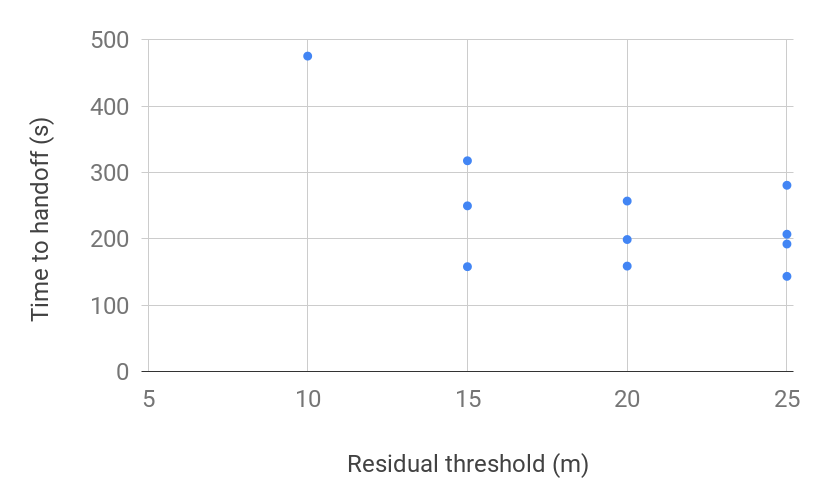
\includegraphics[width=0.7\columnwidth]{figures/sim_threshold_vs_time}
  \caption{Negative relationship between residual threshold and time to handoff for various window size values.}
  \label{fig:sim_threshold_vs_time}
\end{figure}



%We also increased the sensor noise parameters for the simulated range and magnetometer measurements to see how increased noise would affect the performance of the full system. Interestingly, we observed that as we increased the standard deviation of the noise, the performance of the system increased slightly up to a point, then degraded as the noise was increased further, as seen in Figure\stcomment{add plot}. It seems as though a slight increase in the noise

%a slight increase in the noise for both sensors actually improved the performance of the handoff logic, but
